\chapter{プロセス間通信}
\label{interProcessCommunication}
この章では
プロセス間通信(IPC:Inter-Process Communication)について学ぶ.
\ref{synchronaization}章で学んだ,
「生産者と消費者の問題」や「リーダ・ライタ問題」の具体的な解を得るためには,
プロセス間で情報を共有することが必要である.
プロセス間で情報を共有する代表的な機構として,
\emph{共有メモリ}と\emph{メッセージ通信}がある.

複数のプロセスが情報を共有し協調して処理を進めることで,
次のようなメリットが期待できる.

\begin{itemize}
\item 複数のプロセスが共通の情報へアクセスすることができる.
\item 並列処理による処理の高速化ができる可能性がある.
\item システムを見通しの良いモジュール化された構造で構築できる.
\end{itemize}

%==============================================================================
\section{共有メモリ}
共有メモリは\figref{ipcShearedMemory}に示すように,
プロセス間で同じ物理メモリを共有する方式である.
プロセス1とプロセス2は同じ物理メモリ(共有メモリ)を,
それぞれの仮想メモリ空間に貼り付けている.

\begin{myfig}{btp}{共有メモリ}{ipcShearedMemory}
  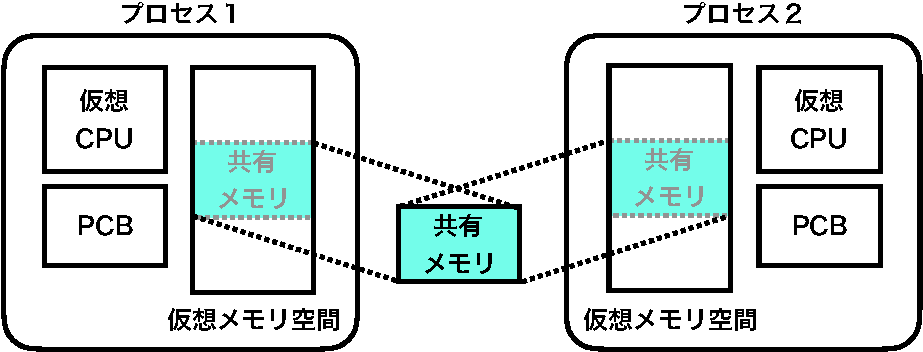
\includegraphics[scale=0.6]{Fig/ipcShearedMemory-crop.pdf}
\end{myfig}

メモリ管理のハードウェア(Memory Management Unit : MMU)\footnote{
  MMUに付いては第\ref{memoryManagement}部「メモリ管理」で解説する.
}を適切に設定することで,
複数のプロセスの仮想メモリ空間に同じ物理メモリを貼り付ける.
メモリを貼り付ける操作はシステムコールを用いて行う.
貼り付けが完了した後は,
システムコールを用いることなく情報の共有が可能であるが,
プロセス間の同期機構は別に準備する必要がある.

\subsection{UNIXの共有メモリ関連システムコール等}
UNIXの共有メモリ関連のシステムコールとライブラリ関数を
\figref{ipcUnixShearedMemory}に紹介する.

\begin{myfig}{btp}{UNIXの共有メモリ関連システムコールとライブラリ関数}
  {ipcUnixShearedMemory}
  \lstinputlisting[numbers=none]{Lst/ipcUnixShearedMemory.txt}
\end{myfig}

\begin{quote}
  \begin{description}
  \item [\texttt{ftok()}ライブラリ関数]
    \|ftok()|は,\|path|と\|id|の組合せからから,
    システム内で一意かつ唯一の\|key|値を生成する.

  \item [\texttt{shmget}システムコール]
    \|key|値で識別される共有メモリセグメントのID返す.
    \|key|値で識別される共有メモリセグメントが存在しない場合は,
    \|size|バイトのものを新しく作ることも可能である.
    \|flag|の値は共有メモリのアクセス許可ビット(\|rwxrwxrwx|)と,
    \|IPC_CREAT|等のフラグである.

  \item [\texttt{shmat}システムコール]
    共有メモリセグメントをID(\|shmId|)で指定し,
    プロセスの仮想アドレス空間に貼り付ける.

  \item [\texttt{shmdt}システムコール]
    共有メモリセグメントをID(\|shmId|)で指定し,
    プロセスの仮想アドレス空間から取り除く.

  \item [\texttt{shmctl}システムコール]
    共有メモリセグメントをID(\|shmId|)で指定し操作する.
    共有メモリセグメントの削除等の操作ができる.
  \end{description}
\end{quote}

\subsection{UNIXの共有メモリ使用例}
共有メモリセグメントを作成し,
そこから定期的にデータを読み出し表示するサーバプログラムの例を
リスト\ref{ipcUnixShearedMemoryServer}に示す\footnote{
  ここで示すプログラムは macOS 10.13.2 で動作確認してあるが,
  他のUNIXでも動作するはずである.}.
また,サーバプログラムが作成した共有メモリセグメントにデータを書き込む
クライアントプログラムの例を
リスト\ref{ipcUnixShearedMemoryClient}に示す.

\lstinputlisting[numbers=left,float=btp,label=ipcUnixShearedMemoryServer,
  caption=UNIXの共有メモリサーバ例]{Lst/ipcUnixShearedMemoryServer.c}

\lstinputlisting[numbers=left,float=btp,label=ipcUnixShearedMemoryClient,
  caption=UNIXの共有メモリクライアント例]{Lst/ipcUnixShearedMemoryClient.c}

サーバプログラムでは,
28行の\|printf()|が共有メモリ(\|data|)から文字列を読み出し表示する.
文字列が\|end|ならプログラムを終了する.
クライアントプログラムでは,
27行の\|fgets()|が共有メモリ(\|data|)に文字列を書き込む.
これらのプログラムでは,
共有メモリが普通の文字配列のように\|printf()|や\|fgets()|に渡されている.
共有メモリなので,
\|fgets()|が書き込んだ内容を\|printf()|が読み出すことになる.

実行例は\figref{ipcUnixShearedMemoryTest}のようになる.
図は二つのターミナルを開いて操作した状態を示している.
左半分が第一のターミナル,
右半分が第二のターミナルである.
まず,左のターミナルで
サーバプログラム(ipcUnixShearedMemoryServer)を起動する.
これで共有メモリセグメントが準備された.
次に,右のターミナルで
クライアントプログラム(ipcUnixShearedMemoryClient)を起動する.
この状態で右のターミナルに入力した文字列が,
クライアントプログラムにより共有メモリに書き込まれる.
左のターミナルで実行中のサーバプログラムは,
共有メモリの内容を定期的に表示する.

\begin{myfig}{btp}{UNIXのメモリ共有プログラム実行例}{ipcUnixShearedMemoryTest}
  \lstinputlisting[numbers=none]{Lst/ipcUnixShearedMemoryTest.txt}
\end{myfig}

ここに紹介した簡単なプログラムでは,
クライアントプロセスがデータを書き換え中に,
サーバプロセスがデータを読み出す可能性がある.
\emph{このようなプログラムを使用してはならない.}
実際に使用する場合は書き換え中のデータを読み出さないように,
セマフォ等\footnote{UNIXではセマフォも使用できる.}を
用いて相互排除を行う必要がある.
原理の確認以外の目的に\emph{このプログラムを使用してはならない.}

%==============================================================================
\section{メッセージ通信}
メッセージ通信は\figref{ipcMessagePassing}に示すように,
システムコールを用いてプロセス間で情報をコピーする方式である.
プロセス1は\|send()|システムコールを用いて
プロセス2へメッセージを送る.
プロセス2は\|receive()|システムコールを用いて
プロセス1からメッセージを受取る.

\begin{myfig}{btp}{メッセージ通信}{ipcMessagePassing}
  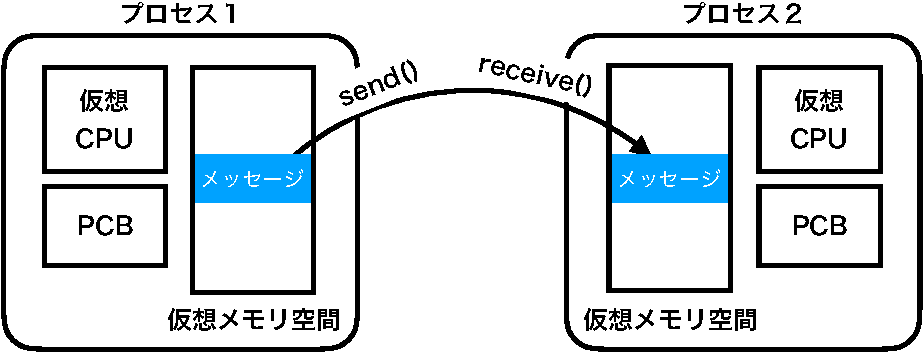
\includegraphics[scale=0.6]{Fig/ipcMessagePassing-crop.pdf}
\end{myfig}

メッセージ通信は,
データを送る度にシステムコールを使用するのでオーバーヘッドが大きいが,
プロセス間の同期機構としても働く.

\subsection{通信相手の指定方式(Naming)}
メッセージの通信相手を指定する方式が二つある.

\begin{quote}
  \begin{description}
  \item[直接指定方式]
    相手プロセスを直接指定する方式である.
    \figref{ipcDirect}は直接指定方式を表している.

    \begin{myfig}{btp}{直接指定方式}{ipcDirect}
      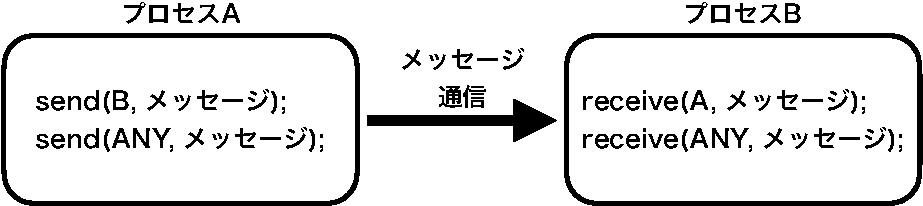
\includegraphics[scale=0.6]{Fig/ipcDirect-crop.pdf}
    \end{myfig}

    \|send()|,\|receive()|システムコールの引数は,
    \emph{相手プロセス}と\emph{メッセージ}になる.
    \emph{相手プロセス}として\|ANY|のような記述を許すことで,
    多対多の通信も可能である.
    また,受信したメッセージをいくつか貯めることが可能な,
    バッファ付きの通信方式もあり得る.

  \item[間接指定方式]
    \emph{リンク(ポート,ソケット,チャネルとも呼ばれる)}を作成し,
    通信先としてリンクの名前を用いる方式である.
    \figref{ipcIndirect}は間接指定方式を表している.

    \begin{myfig}{btp}{間接指定方式}{ipcIndirect}
      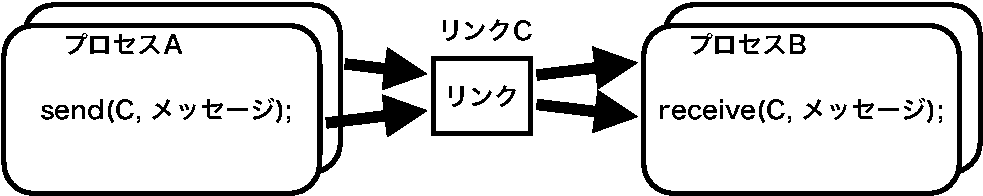
\includegraphics[scale=0.6]{Fig/ipcIndirect-crop.pdf}
    \end{myfig}

    \|send()|,\|receive()|システムコールの引数は,
    \emph{リンク}と\emph{メッセージ}になる.
    同じリンクを共有する複数のプロセスが存在すると,
    自然に多対多の通信方式が実現できる.
    リンクにメッセージをいくつか貯めるバッファ機能を持たせる場合が多い.
    %UNIXのソケットやパイプはこの方式によく似ている.
  \end{description}
\end{quote}

\subsection{バッファリング(Buffering)}
直接指定方式か間接指定方式かに関わりなく,
メッセージを格納するバッファを用意することができる.
送信プロセスはバッファに空きがあれば待ち時間なしに
\|send()|システムコールを完了できる.
受信プロセスはバッファにメッセージがあれば待ち時間なしに
\|receive()|システムコールを完了できる.

間接指定方式ではリンクがバッファを持つと考え,
リンクを作成する時点でバッファの大きさを指定する場合が多い.
\figref{ipcIndirect}で「リンク」の位置にバッファがあると考えると分かりやすい.

\subsection{メッセージの形式}
通信に用いられるメッセージの形式には次のような選択肢がある.

\begin{quote}
  \begin{description}
  \item [メッセージ長] \emph{固定長方式}または\emph{可変長方式}
  \item [メッセージ形式] \emph{タグ付き}または\emph{タグなし}
  \end{description}
\end{quote}

\emph{タグ}は種類を表すためにメッセージに付加されるデータのことである.
タグ付きのメッセージ通信機構では,
送信側はメッセージにタグを付加する.
受信側はタグを指定してメッセージを選択的に受信することができる.

\subsection{同期方式(Synchronization)}
\emph{非同期方式(ノンブロッキング:Nonblocking)}と
\emph{同期方式(ブロッキング:Blocking)}の二つがある.
同期式の特別な場合としてバッファを用いない\emph{ランデブー方式}も考えられる.

\begin{quote}
  \begin{description}
  \item [非同期方式]
    \|send()|はバッファに空きがない場合エラーで終了する.
    \|receive()|はバッファにメッセージがない場合エラーで終了する.
  \item [同期方式]
    \|send()|はバッファに空きがない場合ブロックし空きができるのを待つ.
    \|receive()|はバッファにメッセージがない場合ブロックし
    メッセージが届くのを待つ.
  \item [ランデブー方式]
    \|send()|は受信プロセスが\|receive()|を実行するまでブロックする.
    \|receive()|は送信プロセスが\|send()|を実行するまでブロックする.
    両方のプロセスが\|send()|と\|receive()|を
    実行したらプロセス間でメッセージをコピーする.
    プロセス間で直にメッセージをコピーするので,
    バッファは不要である.
  \end{description}
\end{quote}

\subsection{UNIXのメッセージ通信システムコール}
UNIXでは複数種類のメッセージ通信機構が利用可能である.
ここでは,System V 系のUNIXを起原とする方式を紹介する.
この方式は,\emph{間接指定方式},\emph{バッファリングあり},
\emph{可変長},\emph{タグ付き}の方式である.
システムコールの引数によって,
\emph{同期方式}と\emph{非同期方式}のどちらにも対応することができる.
UNIXのメッセージ通信関連のシステムコール等を\figref{ipcUnixMessage}に示す.

\begin{myfig}{btp}{UNIXのメッセージ通信関連システムコールとデータ構造}
  {ipcUnixMessage}
  \lstinputlisting[numbers=none]{Lst/ipcUnixMessage.txt}
\end{myfig}

\begin{quote}
  \begin{description}
  \item [\texttt{msgBuf}構造体]
    ユーザが宣言する構造体である.
    必ず,long型の\|mtype|フィールドから始める必要がある.
    このフィールドが\emph{タグ}の役割を持つ.
    \|mtext|はメッセージの本体を格納する領域であり,
    ユーザが自由に大きさや用途を決めることができる.
  \item [\texttt{msgget()}システムコール]
    リンク(メッセージキューと呼ぶ)のIDを返す.
    \|key|は,共有メモリの場合と同様に\|ftok()|関数を用いて生成した値である.
    メッセージキューを識別するために用いる.
    \|msgflg|に\|IPC_CREAT|を指定することで,
    メッセージキューを新規に作成することもできる.
  \item [\texttt{msgsnd()}システムコール]
    \|msqid|で指定したメッセージキューにメッセージを送信する.
    \|msgp|に送信するメッセージを格納した\|msgBuf|構造体のポインタを渡す.
    メッセージは\emph{可変長方式}なので\|msgsz|で長さを指定する.
    \|msgsz|は構造体全体ではなく,構造体の\|mtext|部分のバイト数である.
    \|msgflg|に\|IPC_NOWAIT|フラグを指定すると\emph{非同期方式}になり,
    指定しないと\emph{同期方式}になる.
  \item [\texttt{msgrcv()}システムコール]
    \|msqid|で指定したメッセージキューからメッセージを受信する.
    \|msgp|に受信したメッセージを格納する\|msgBuf|構造体のポインタを渡す.
    \|msgsz|は受信可能な\|mtext|の最大バイト数である.
    \|msgtyp|に受信したいメッセージの\|mtype|を指定し,
    \emph{タグ}が合致するメッセージを選択的に受信できる.
    \|msgflg|に\|IPC_NOWAIT|フラグを指定すると\emph{非同期方式}になる.
  \item [\texttt{msgclt()}システムコール]
    \|msqid|で指定したメッセージキューに対して操作を行う.
    \|cmd|に操作の種類(コマンド),
    \|buf|にパラメータを渡す.
    \|IPC_RMID|コマンドを指定するとメッセージキューの削除ができる.
  \end{description}
\end{quote}

\subsection{UNIXのメッセージ通信プログラム例}
メッセージを表現する構造体の例をリスト\ref{ipcUnixMessageH}に示す\footnote{
  ここで紹介するプログラムはmacOS 10.13.2 で動作確認した.
  macOSのオンラインマニュアルには,
  ここで紹介するメッセージ通信方式について記載がないが,
  試してみると使用できた.}.
メッセージ本体の長さは\|MAXMSG|に定義している.
以下のプログラムは,メッセージ長をこの値に固定した例になっている.

\lstinputlisting[caption=UNIXのメッセージ通信プログラム例(メッセージ構造体),
  numbers=left,float=btp,label=ipcUnixMessageH]{Lst/ipcUnixMessage.h}

リスト\ref{ipcUnixMessageWriter}に
メッセージキューを作成しメッセージを書き込むプログラムの例を示す.
このプログラムは入力した文字列をメッセージ本体に格納して
メッセージキューに送信する.
タグの役割を持つ\|mtype|は常に1にしている.

\lstinputlisting[numbers=left,float=btp,label=ipcUnixMessageWriter,
  caption=UNIXのメッセージ通信プログラム例(メッセージ送信側)]
                {Lst/ipcUnixMessageWriter.c}

リスト\ref{ipcUnixMessageReader}に,
メッセージキューからメッセージを読み込み内容を表示するプログラムの例を示す.
22行で\|msgtyp|を0にして\|msgrcv()|を実行している.
\|msgtyp|が0の場合は,
メッセージの\|mtype|(タグ)を無視して
メッセージキューの先頭から順にメッセージを受信する.
26行で\|mtype|と\|mtext|の内容を表示している.
送信側のプログラムがメッセージキューを削除すると
22行でエラーが発生し24行で終了する.

\lstinputlisting[numbers=left,float=btp,label=ipcUnixMessageReader,
  caption=UNIXのメッセージ通信プログラム例(メッセージ受信側)]
                {Lst/ipcUnixMessageReader.c}

\subsection{UNIXのメッセージ通信プログラムの実行例}
メッセージ通信プログラムの実行例を
\figref{ipcUnixMessageTest}に示す.
図は二つのターミナルを開いて操作した状態を示している.
左半分が第一のターミナル,
右半分が第二のターミナルである.
まず,左のターミナルで送信プログラム(ipcUnixMessageWriter)を起動する.
これでメッセージキューが準備された.
次に,右のターミナルで受信プログラム(ipcUnixMessageReader)を起動する.
この状態で左のターミナルに入力した文字列が,
メッセージ通信を用いて右のターミナルで実行中のプログラムに送信される.
右のターミナルには
受信したメッセージの\|mtype|と\|mtext|の内容が表示される.

\begin{myfig}{btp}{UNIXのメッセージ通信プログラム実行例}{ipcUnixMessageTest}
  \lstinputlisting[numbers=none]{Lst/ipcUnixMessageTest.txt}
\end{myfig}

%==============================================================================
\section{メッセージ通信機構の実装例}
第\ref{tacosIPC}章に
TacOSにおけるメッセージ通信機構の実装例を紹介する.
TacOSのメッセージ通信機構はセマフォを利用して実装されている.

%==============================================================================
\section{まとめ}
この章ではプロセス間通信(IPC)について学んだ.
IPCには共有メモリとメッセージ通信の二種類があった.
UNIXの共有メモリとメッセージ通信についてプログラム例を示した.

%==============================================================================
\section*{練習問題}
\begin{enumerate}
  \renewcommand{\labelenumi}{\ttfamily\arabic{chapter}.\arabic{enumi}}
  \setlength{\leftskip}{1em}
\item 次の言葉の意味を説明しなさい.
  \begin{enumerate}
  \item 共有メモリ
  \item メッセージ通信
  \item 直接指定方式
  \item 間接指定方式
  \item バッファリング
  \item 同期方式
  \item 非同期方式
  \item ランデブー方式
  \item メッセージのタグ
  \end{enumerate}
\item プロセス間の共有メモリとスレッド間の共有変数の違いは何か?
\item UNIXの共有メモリ使用例
  (リスト\ref{ipcUnixShearedMemoryServer},
    リスト\ref{ipcUnixShearedMemoryClient})
  を実際に実行し動作確認しなさい.
  なお,ソースプログラムは以下から入手可能である. \\
  \url{https://github.com/tctsigemura/OSTextBook/blob/master/Lst/ipcUnixShearedMemoryServer.c} (サーバ側)\\
  \url{https://github.com/tctsigemura/OSTextBook/blob/master/Lst/ipcUnixShearedMemoryClient.c} (クライアント側)
\item 動作確認したプログラムでは,
  サーバプログラムは共有メモリが変更されたことを確認しないで,
  一定の時間間隔で共有メモリの内容を表示している.
  \begin{enumerate}
  \item どのような不都合が予想されるか?
  \item クライアントとサーバで同期をする方法はあるか?
  \end{enumerate}
\item メッセージ通信でバッファを大きくすることのメリットは何か?
\item UNIXのメッセージ通信プログラム例(リスト\ref{ipcUnixMessageH},
  リスト\ref{ipcUnixMessageWriter},リスト\ref{ipcUnixMessageReader})
  を実際に実行し動作確認しなさい.
  なお,ソースプログラムは以下から入手可能である. \\
  \url{https://github.com/tctsigemura/OSTextBook/blob/master/Lst/ipcUnixMessage.h}(ヘッダファイル)\\
  \url{https://github.com/tctsigemura/OSTextBook/blob/master/Lst/ipcUnixMessageWriter.c}(送信側)\\
  \url{https://github.com/tctsigemura/OSTextBook/blob/master/Lst/ipcUnixMessageReader.c}(受信側)
\item UNIXのメッセージ通信プログラム例は生産者と消費者の問題の解になっている.
  複数生産者と複数消費者の問題の解にもなっているか?
\item UNIXのメッセージ通信プログラム例が
  複数生産者と複数消費者の問題の解にもなっているか,
  動作確認する手順を説明しなさい.
\end{enumerate}
